%-----------------------------------------------------------------------------------------------------------------------------------------------%
%	The MIT License (MIT)
%
%	Copyright (c) 2021 Jitin Nair
%
%	Permission is hereby granted, free of charge, to any person obtaining a copy
%	of this software and associated documentation files (the "Software"), to deal
%	in the Software without restriction, including without limitation the rights
%	to use, copy, modify, merge, publish, distribute, sublicense, and/or sell
%	copies of the Software, and to permit persons to whom the Software is
%	furnished to do so, subject to the following conditions:
%	
%	THE SOFTWARE IS PROVIDED "AS IS", WITHOUT WARRANTY OF ANY KIND, EXPRESS OR
%	IMPLIED, INCLUDING BUT NOT LIMITED TO THE WARRANTIES OF MERCHANTABILITY,
%	FITNESS FOR A PARTICULAR PURPOSE AND NONINFRINGEMENT. IN NO EVENT SHALL THE
%	AUTHORS OR COPYRIGHT HOLDERS BE LIABLE FOR ANY CLAIM, DAMAGES OR OTHER
%	LIABILITY, WHETHER IN AN ACTION OF CONTRACT, TORT OR OTHERWISE, ARISING FROM,
%	OUT OF OR IN CONNECTION WITH THE SOFTWARE OR THE USE OR OTHER DEALINGS IN
%	THE SOFTWARE.
%	
%
%-----------------------------------------------------------------------------------------------------------------------------------------------%

%----------------------------------------------------------------------------------------
%	DOCUMENT DEFINITION
%----------------------------------------------------------------------------------------

% article class because we want to fully customize the page and not use a cv template
\documentclass[a4paper,12pt]{article}

%----------------------------------------------------------------------------------------
%	FONT
%----------------------------------------------------------------------------------------

% % fontspec allows you to use TTF/OTF fonts directly
% \usepackage{fontspec}
% \defaultfontfeatures{Ligatures=TeX}

% % modified for ShareLaTeX use
% \setmainfont[
% SmallCapsFont = Fontin-SmallCaps.otf,
% BoldFont = Fontin-Bold.otf,
% ItalicFont = Fontin-Italic.otf
% ]
% {Fontin.otf}

%----------------------------------------------------------------------------------------
%	PACKAGES
%----------------------------------------------------------------------------------------
\usepackage{url}
\usepackage{parskip} 
%\usepackage[english]{babel}
\usepackage{csquotes}

%other packages for formatting
\RequirePackage{color}
\RequirePackage{graphicx}
\usepackage[dvipsnames]{xcolor}
\usepackage[scale=0.85]{geometry}

%tabularx environment
\usepackage{tabularx}

%for lists within experience section
\usepackage{enumitem}

% centered version of 'X' col. type
\newcolumntype{C}{>{\centering\arraybackslash}X} 

%to prevent spillover of tabular into next pages
\usepackage{supertabular}
\usepackage{tabularx}
\newlength{\fullcollw}
\setlength{\fullcollw}{0.47\textwidth}

%custom \section
\usepackage{titlesec}				
\usepackage{multicol}
\usepackage{multirow}
\usepackage{tikz}
\usepackage{tikzpagenodes}
\usetikzlibrary{calc}

%CV Sections inspired by: 
%http://stefano.italians.nl/archives/26
\titleformat{\section}{\Large\scshape\raggedright}{}{0em}{}[\titlerule]
\titlespacing{\section}{0pt}{10pt}{10pt}

%%%%%
%for publications
%\usepackage[style=authoryear,sorting=ynt, maxbibnames=2, backend=biber]{biblatex}

%Setup hyperref package, and colours for links
\usepackage[unicode, draft=false]{hyperref}
\definecolor{linkcolour}{rgb}{0,0.2,0.6}
\hypersetup{colorlinks,breaklinks,urlcolor=linkcolour,linkcolor=linkcolour}
%\addbibresource{citations.bib}
%\setlength\bibitemsep{1em}
%%%%%

%for social icons
\usepackage{fontawesome5}

%debug page outer frames
%\usepackage{showframe}

%----------------------------------------------------------------------------------------
%	BEGIN DOCUMENT
%----------------------------------------------------------------------------------------
\begin{document}

% non-numbered pages
\pagestyle{empty} 

%----------------------------------------------------------------------------------------
%	TITLE
%----------------------------------------------------------------------------------------

% \begin{tabularx}{\linewidth}{ @{}X X@{} }
% \huge{Your Name}\vspace{2pt} & \hfill \emoji{incoming-envelope} email@email.com \\
% \raisebox{-0.05\height}\faGithub\ username \ | \
% \raisebox{-0.00\height}\faLinkedin\ username \ | \ \raisebox{-0.05\height}\faGlobe \ mysite.com  & \hfill \emoji{calling} number
% \end{tabularx}
{\Huge \textbf{Curriculum Vitae --\\[0.3cm]}} 
{\Large \textit{Oscar Stommendal}} \\[0.2cm]
\begin{tabular}[c]{l | l}
    \href{mailto:oscar.stommendal01@gmail.com}{\raisebox{-0.05\height}\faEnvelope \ Email}& \hspace{0.10cm}
    \href{https://github.com/stommen} {\raisebox{-0.05\height}\faGithub \ Github}\\ \href{tel:+46706617353}{\raisebox{-0.05\height}\faMobile \ iPhone} &
    \hspace{0.10cm} \href{https://stommen.github.io}{\raisebox{-0.05\height}\faGlobe \ Personal Webpage} \\
    \href{https://linkedin.com/in/oscar-stommendal} {\raisebox{-0.05\height}\faLinkedin\ LinkedIn}& 
    \hspace{0.15cm} \href{https://www.google.se/maps/place/Chalmers+tekniska+högskola/@57.6898004,11.9715868,17z/data=!3m1!4b1!4m6!3m5!1s0x464ff36b628efec3:0xc148ed83d6f0a03!8m2!3d57.6898004!4d11.9741617!16zL20vMDFxam0?entry=ttu&g_ep=EgoyMDI0MDkwOS4wIKXMDSoASAFQAw%3D%3D}{\raisebox{-0.05\height}\faMapMarker \ Chalmers University of Technology}
\end{tabular}
\hspace{5cm}
\begin{tikzpicture}[remember picture,overlay]
\clip ($(current page text area.north east)!0.075!(current page text area.south east)!0.12!(current page text area.north west)$)
  circle (1.9cm) node {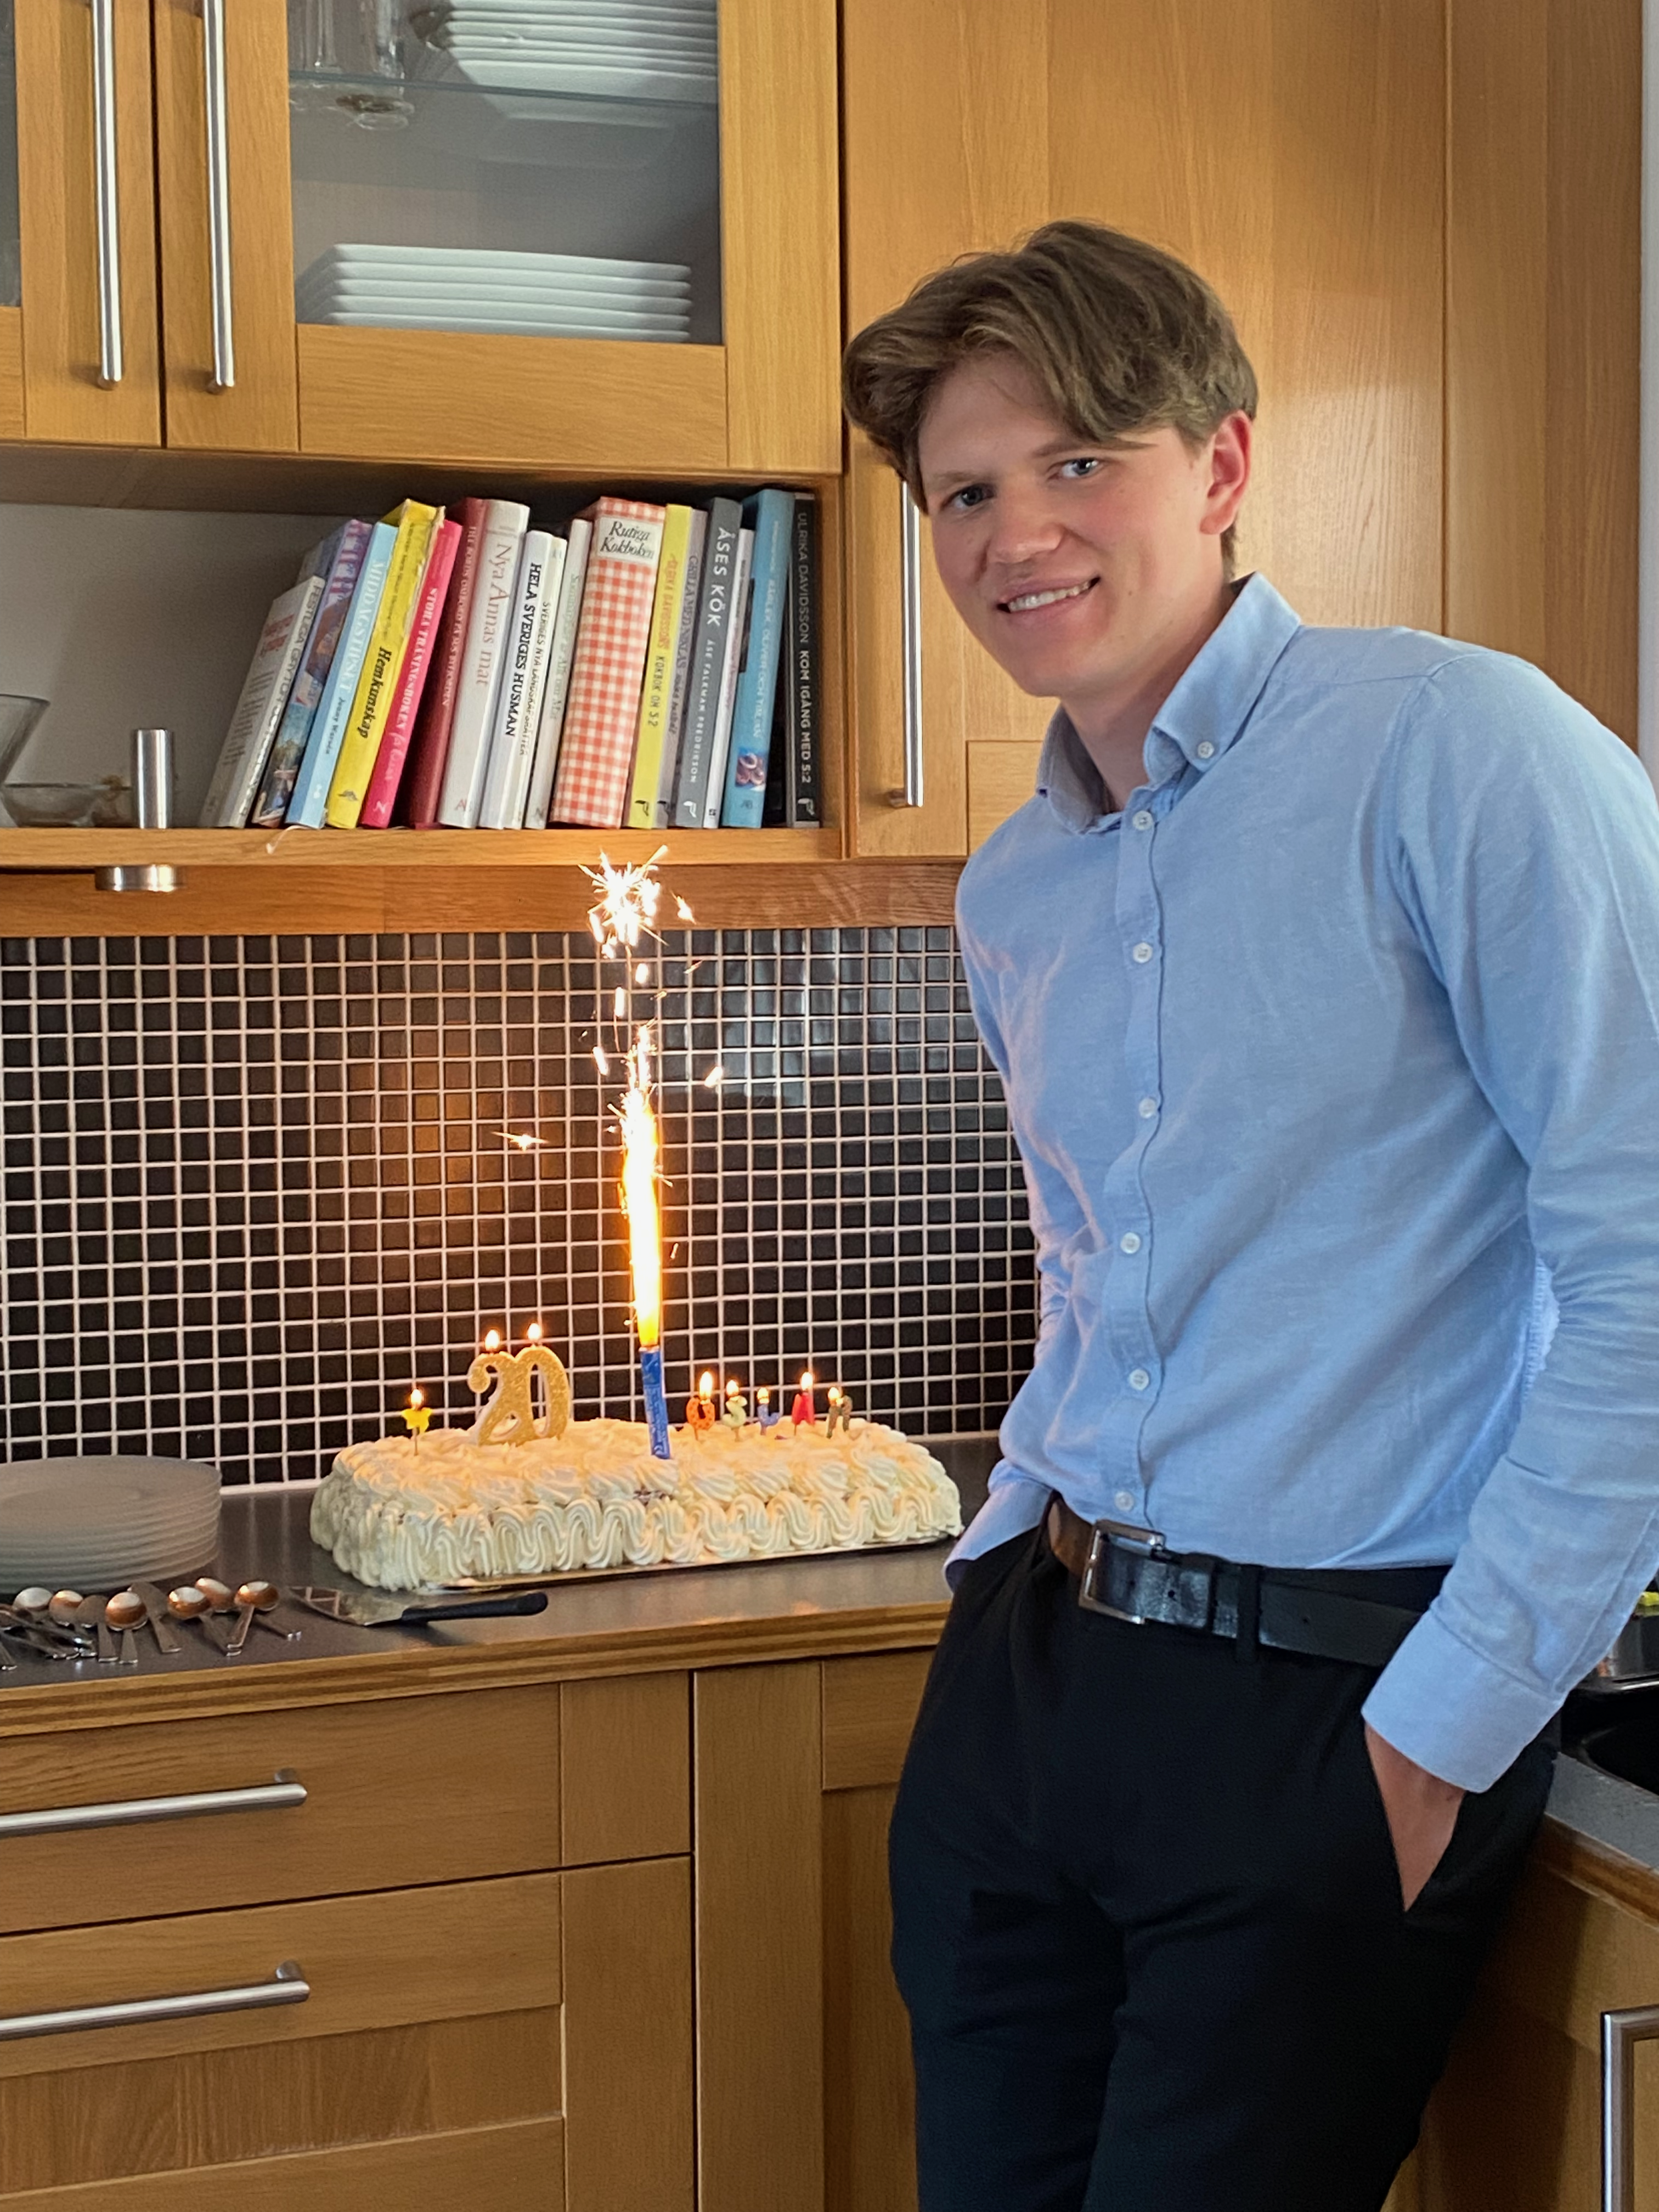
\includegraphics[width=3.8cm]{cv_bild.pdf}};
\end{tikzpicture}
\hspace*{0.1cm}\\[0.1cm]
%\begin{tabularx}{\linewidth}{@{} C @{}}
%\Huge{Oscar Stommendal} \\[7.5pt]
%\href{https://linkedin.com/in/oscarstommendal}{\raisebox{-0.05\height}\faLinkedin\ oscarstommendal} \ $|$ \ 
%\href{mailto:oscar.stommendal01@gmail.com}{\raisebox{-0.05\height}\faEnvelope \ oscar.stommendal01@gmail.com} \ $|$ \ 
%href{tel:+46706617353}{\raisebox{-0.05\height}\faMobile \ +46 70-661-7353} \\
%\end{tabularx}
%----------------------------------------------------------------------------------------
% EXPERIENCE SECTIONS
%----------------------------------------------------------------------------------------
%Interests/ Keywords/ Summary
\section{Goal with application}

% In english:
\section{Main competences}
\begin{itemize}
    \item[*] Practical experience of engineering work (mainly in programming) through internships
    \item[*] Analytical and methodical
    \item[*] (Collaborative) Programming: Python, Git and Matlab
    \item[*] Goal-oriented and competitive -- hence very result-oriented
    \item[*] Calm and planning
\end{itemize}

%	EDUCATION
%----------------------------------------------------------------------------------------
\section{Education}
\begin{tabularx}{\linewidth}{@{}l X@{}}	
2024 - now &MSc in Physics på \textbf{Chalmers University of Technology} \hfill \\
&Focus on computational physics, astronomy and quantum physics. \\
&\textit{Including an exchange semester at} \textbf{Nanyang Technological University}, \textit{Singapore.} \\[5pt] 

2023 - now &BSc in Business and Economics at \textbf{Gothenburg University} \hfill \\[5pt] 

2020 - 2023 &BSc in Engineering Physics på \textbf{Chalmers University of Technology} \hfill \\[5pt] 

2017 - 2020 &Natural Sciences program at \textbf{Nils Ericsonsgymnasiet} \hfill \\ 
\end{tabularx}

%----------------------------------------------------------------------------------------

%Experience
\section{Work experience}

\begin{tabularx}{\linewidth}{ @{}l r@{} }
\textbf{Summer work @ \textit{Norra Älvsborgs Länssjukhus (NÄL)}} & \hfill Jul 2019 - Aug 2019 \\[5pt]
\multicolumn{2}{@{}X@{}}{Kitchen responsibility at the X-ray department. I also got to see a lot of the work on the department.} \\[10.75pt]
%\end{tabularx}

%\begin{tabularx}{\linewidth}{ @{}l r@{} }
\textbf{Summer work @ \textit{ICA Supermarket Mellerud}} & \hfill Jun 2020 - Aug 2022 \\[5pt]
\multicolumn{2}{@{}X@{}}{Cashier responsibilities, goods unpacking and charcuterie. I also got to mentor new starters. This was a valuable experience since I got to meet and handle lots of different people.} \\[10.75pt]
\end{tabularx}

\begin{tabularx}{\linewidth}{ @{}l r@{} }
    \textbf{Part-time consultant @ \textit{Nordisk rörmärkning AB}} & \hfill Apr 2021 - Nov 2023 \\[3.75pt]
    \multicolumn{2}{@{}X@{}}{
    \begin{minipage}[t]{\linewidth}
        Solved different tasks to make the company's website and customer orders more efficient and automated through Excel. Here I learned to use basic Visual Basic.
    \end{minipage}
    }
    \end{tabularx}

\begin{tabularx}{\linewidth}{ @{}l r@{} }
\textbf{Summer internship in the GTC-department -- \textit{GKN Aerospace}} & \hfill Jun 2023 - Aug 2023 \\[3.75pt]
\multicolumn{2}{@{}X@{}}{
\begin{minipage}[t]{\linewidth}
    Department of product integration and simulation. The work mostly consisted of programming in Python,
    where I simplified and automated data collection for test runs within a certain project, and created a 
    program to execute stress calculations on bodies created in ANSYS (CAD).
\end{minipage}}
\end{tabularx}

\begin{tabularx}{\linewidth}{ @{}l r@{} }
\textbf{Research Technician - Digital simulation and analysis -- \textit{GKN Aerospace}} & \hfill Sep 2023 - now \\[3.75pt]
\multicolumn{2}{@{}X@{}}{
\begin{minipage}[t]{\linewidth}
    I got the opportunity to extend the contract at GKN as a Research Technician. I worked partly in Matlab for automatic data collection during test runs within a certain project, where I improved and streamlined the code, and developed it to analyze more data. I also developed a package in Python that can be used internally at GKN to create and edit so-called Quality Assurance documents, which ensure the quality and use of a software or package.
\end{minipage}}
\end{tabularx}

%----------------------------------------------------------------------------------------
%	SKILLS
%----------------------------------------------------------------------------------------
%----------------------------------------------------------------------------------------
\section{Skills and Qualifications}

\begin{tabularx}{\linewidth}{ @{}l r@{} }
\textbf{Programmering and software} \\[3.75pt]
\multicolumn{2}{@{}X@{}}{
\begin{minipage}[t]{\linewidth}
\begin{itemize}
    \item[--] \textit{Very good knowlegde}: Microsoft office (except Access), Python, Matlab, Github, Git
    \item[--] \textit{Good knowledge}: Latex, Linux, Azure
    \item[--] \textit{Basic knowlegde}: HTML, YAML, Labview, ANSYS, Visual Basic
\end{itemize}
\vspace{0.1cm}
    \end{minipage}
}
\end{tabularx}

\begin{tabularx}{\linewidth}{ @{}l r@{} }
\textbf{Personal traits} \\[3.75pt]
\multicolumn{2}{@{}X@{}}{
\begin{minipage}[t]{\linewidth}
\begin{itemize}
    \item[--] Calm, humble and planning
    \item[--] Team player
    \item[--] Caring  
    \item[--] Always positive and cheerful
    \item[--] Very driven, goal-oriented (stubborn) and competitive  
\end{itemize}
\end{minipage}
}
\end{tabularx}

\begin{tabularx}{\linewidth}{ @{}l r@{} }
\textbf{Language} \\[3.75pt]
\multicolumn{2}{@{}X@{}}{
\begin{minipage}[t]{\linewidth}
\begin{itemize}
    \item[--] Swedish: Native language
    \item[--] English: Fluent
    \item[--] Spanish: Basic knowledge   
\end{itemize}
    \end{minipage}
}
\end{tabularx}

\section{Other qualifications}
\begin{tabularx}{\linewidth}{@{}l X@{}}	
2022 & Qualified for membership in \textbf{MENSA} Sweden \hfill \\[10.75pt]
2019 & \textbf{Driver's license}, B \hfill \\ \\
\end{tabularx}
\textit{References/certificates/grades will be provided upon request}.
\vfill
\center{\footnotesize Latest updated: \today \\
CV created in \LaTeX

\end{document}